\chapter{Implementierung}

\section{Laden und Aufbereitung der MNIST Daten}
Für das Neuronale Netzwerk zur Erkennung von hangeschriebenen Zeichen zwischen werden Test- und Trainingsdaten der MNIST Datenbank genutzt. Die Datensätze können unter folgender Adresse gefunden werden: 
\\[0.2cm]
\hspace*{1.3cm}
\href{http://yann.lecun.com/exdb/mnist/}{http://yann.lecun.com/exdb/mnist/}
\\[0.2cm]
Da der MNIST Datensatz lediglich in Form von Binärdateien vorliegt und es in der aktuellen Version von SetlX nicht möglich ist Binärdateien zu lesen, wurde statt dem original Datensatz der umgewandelte Datensatz in Form einer CSV-Datei verwendet. Die Dateien können hier heruntergeladen werden:
\\[0.2cm]
\hspace*{1.3cm}
\href{https://pjreddie.com/projects/mnist-in-csv/}{https://pjreddie.com/projects/mnist-in-csv/}
\\[0.2cm]
Die Verwendung des CSV-Formats führt dazu, dass die Größe der Datensätze auf Grund fehlender Komprimierungen ansteigt. Ebenso wird das Einlesen der Datensätze langsamer, was an der eigentlichen Funktion des neuronalen Netzes allerdings nichts ändert und somit für dieses Projekt vertretbar ist. \\
Verwendet werden die CSV-Dateien $\mathtt{mnist\_test.csv}$ und $\mathtt{mnist\_train.csv}$. Die Traingsdaten umfassen insgesamt 60.000 Datensätze und die Testdaten 10.000 Datensätze. 
Die einzelnen Datensätze, also die handgeschriebenen Zeichen, sind in den Dateien in folgendem Format gespeichert:
\begin{center}
	$\mathtt{label1, pixel11, pixel12, pixel13, ...}$ \\
	$\mathtt{label2, pixel21, pixel22, pixel23, ...}$ \\
	...
\end{center}
Hierbei bezeichnet Label den Wert der jeweils gezeichneten Ziffer (wird benötigt um zu überprüfen, ob das Netzwerk die korrekte Ziffer identifiziert hat und um das Netzwerk zu trainieren). \\ \\
Um die Datensätze nun in SetlX importieren zu können, wird die Datei $\mathtt{csv\_loader.stlx}$ verwendet. Wird die Datei im SetlX-Interpreter ausgeführt, so liest sie die CSV-Dateien der Test- und Trainingsdaten (die Dateien müssen im selben Verzeichnis liegen und den oben erwähnten Namen haben) und speichert die Daten in den Variablen $\mathtt{test\_data}$ sowie $\mathtt{training\_data}$. Die Testdaten sind hierbei als Liste von Paaren in Form folgender Form abgelegt: \\
\hspace*{0.3cm}
$
\begin{array}[t]{lcll}
	[ \\[0.1cm]
	
	\hspace*{0.5cm}
	\begin{array}[t]{lcll}
    	[\mathtt{pixels1},\ \mathtt{label1}], \\[0.1cm]
    	[\mathtt{pixels2},\ \mathtt{label2}], \\[0.1cm]
    	... \\[0.1cm]
    \end{array}
    \\[0.1cm]
    
    ] \\[0.1cm]
\end{array}
$
\\[0.0cm]

\noindent
Die Trainingsdaten sind prinzipiell nach dem gleichen Prinzip aufgebaut, allerdings wird hier für spätere Auswertungszwecke der Wert der Ziffer nicht als konkrete Zahl gespeichert, sondern in vektorisierter Form. Der vektorisierte Wert einer Zahl wird hier durch einen Vektor dargestellt, dessen Inhalt immer 0 ist, außer an der $\mathtt{label+1}$-ten Stelle. Dies entspricht dann genau der Form der Ausgabe des Netzwerkes. Beispielhaft würde eine Ziffer mit dem Wert $7$ als folgender Vektor dargestellt werden: \\
$<<0\ 0\ 0\ 0\ 0\ 0\ 0\ 1\ 0\ 0>>$ \\

\noindent
Auf eine genaue Beschreibung der Implementierung des Ladevorgangs wird in dieser Studienarbeit verzichtet, da hierbei keine komplexen Funktionen angewandt wurden und das Verfahren nicht relevant für das Verständnis neuronaler Netze an sich ist.

\section{Implementierung des neuronalen Netzes}
Dieser Abschnitt beschreibt die eigentliche Implementierung des neuronalen Netzwerkes zur Erkennung von handgeschriebenen Ziffern in SetlX. Um den Code möglichst kompakt zu halten, wurden die in den Originaldateien enthaltenen Kommentarzeilen in dieser Seminararbeit zum größten Teil entfernt.
Bei der Umsetzung des Netzwerkes in SetlX wird der SGD-Algorithmus als Lernmethode des Netzwerkes benutzt. Die im vorherigen Kapitel importierten Daten des MNIST-Datensatzes dienen als Grundlage der Ziffernerkennung. 
Das Netzwerk wird als Klasse in SetlX angelegt und enthält die folgenden Membervariablen:

\begin{enumerate}
\item $\mathtt{mNumLayers}$: Anzahl der Layer des aufzubauenden Netzwerkes 
\item $\mathtt{mSizes}$: Aufbau des Layers in Listenform. Bsp.: $[784, 30, 10]$ beschreibt ein Netzwerk mit 784 Inputfeldern, 30 Neuronen im zweiten (hidden) Layer und 10 Output-Neuronen
\item $\mathtt{mBiases}$: Alle Vorbelastungen des Netzwerkes (genauer Aufbau wird im Folgenden erläutert)
\item $\mathtt{mWeights}$: Alle Gewichte des Netzwerkes (genauer Aufbau wird im Folgenden erläutert)
\end{enumerate}

\noindent
Die Initialisierung des Netzwerkes zur Ziffernerkennung erfolgt durch folgende Befehle:
\begin{Verbatim}[ frame         = lines, 
                  framesep      = 0.3cm, 
                  firstnumber   = 1,
                  labelposition = bottomline,
                  numbers       = left,
                  numbersep     = -0.2cm,
                  xleftmargin   = 0.8cm,
                  xrightmargin  = 0.8cm,
                ]
    net := network([784, 30, 10]);
    net.init();
\end{Verbatim}
Als Übergabeparameter bei der Erstellung eines Netzwerk-Objektes wird die Struktur des Netzwerkes in Form einer Liste übergeben. Diese wird dann lediglich $\mathtt{mSizes}$ zugeordnet und basierend hierrauf wird $\mathtt{mNumLayers}$ ermittelt.
Die $\mathtt{init()}$-Funktion der $\mathtt{network}$-Klasse wird verwendet um die Gewichte und Vorbelastungen des Netzwerkes initial zufällig zu belegen. Hiermit werden Ausgangswerte gesetzt, welche später durch das Lernen des Netzwerkes angepasst werden.
Im Folgenden sind die verwendeten Funktionen, welche während der Gewichts- und Vorbelastungs-Initialisierung verwendet werden, zu sehen.
\begin{Verbatim}[ frame         = lines, 
                  framesep      = 0.3cm, 
                  firstnumber   = 1,
                  labelposition = bottomline,
                  numbers       = left,
                  numbersep     = -0.2cm,
                  xleftmargin   = 0.8cm,
                  xrightmargin  = 0.8cm,
                ]
    init := procedure() {
        computeRndBiases();
        computeRndWeights();
    };
    computeRndBiases := procedure() {
        this.mBiases := [ 
            computeRndMatrix([1, mSizes[i]]) : i in [2..mNumLayers] 
        ];
    };
    computeRndWeights := procedure() {
        this.mWeights := [ 
            computeRndMatrix([mSizes[i], mSizes[i+1]]) : i in [1..mNumLayers-1] 
        ];
    };
    computeRndMatrix := procedure(s) {
        [i,j] := s;
        return la_matrix([
            [ ((random()-0.5)*2)/28 : p in [1..i] ] : q in [1..j]
        ]);
    };
\end{Verbatim}

\begin{enumerate}
\item $\mathtt{init()}$: in der init-Funktion werden die Funktionen computeRndBiases() und $\mathtt{computeRndWeights()}$ aufgerufen
\item $\mathtt{computeRndBiases()}$: Die Funktion befüllt die Variable mBiases mit zufälligen Werten. Der für das Netzwerk benötigte Aufbau der Vorbelastungen entspricht folgender Form: \\
$[ \\ 
<<\ <<\mathtt{b\_layer1\_neu1}>>\ <<\mathtt{b\_layer1\_neu2}>>\ ...\ >>, \\
<<\ <<\mathtt{b\_layer2\_neu1}>>\ ...\ >>, \\
 ...\ ]$ \\
Das heißt es kann auf die Vorbelastungen mit folgendem Schema in SetlX zugegriffen werden: \\
\begin{center}
	$\mathtt{mBiases[layer][neuron][bias]}$
\end{center}
Hierbei ist zu beachten, dass der Wert für $\mathtt{bias}$ immer 1 ist, da jedes Neuron nur eine einzige Vorbelastung besitzt. Da es sich bei der Eingabe-Schicht des Netzwerkes nicht um Sigmoid-Neuronen handelt, sondern lediglich um Eingabewerte, werden hierfür keine Vorbelastungen benötigt. Deshalb wird bei der Erstellung der zufälligen Vorbelastungen nur $[2..\mathtt{mNumLayers}]$ (also alle Schichten außer dem Ersten) betrachtet.
\item $\mathtt{computeRndWeights()}$: Diese Funktion ist equivalent zu der Vorbelastungs-Funktion, lediglich wird folgende Struktur der Gewichte angelegt: \\
$[ \\ 
<<\ <<\mathtt{w1\_layer2\_neu1}\ \mathtt{w1\_layer2\_neu2}\ ...\ >>\ << \mathtt{w2\_layer2\_neu1}\ ...\ >>\ ...\ >>, \\
<<\ <<\mathtt{w1\_layer3\_neu1}\  \mathtt{w1\_layer3\_neu2}\ ...\ >>\ <<\mathtt{w2\_layer3\_neu1}\ ...\ >>\ ...\ >>, \\
...\ ]$ \\
Dies entspricht folgenden Zugriffsmöglichkeiten: \\ 
\begin{center}
	$\mathtt{mWeights[layer-1][neuron][weight\ for\ input\ neuron]}$
\end{center}
Der Zugriff auf die Schichten mittels $\mathtt{[layer-1]}$ resultiert aus den fehlenden Gewichten der Eingabe-Schicht.
\item $\mathtt{computeRndMatrix()}$: Diese Hilfsfunktion dient zur Erstellung der Struktur der Gewichte und Vorbelastungen in den zuvor vorgestellten Funktionen. Die Funktion enthält als Parameter eine Matrix-Struktur in Listenform und liefert die zugehörige Matrix mit zufälligen Werten zwischen $-1/28$ und $1/28$ zurück. Der Wert 28 ergibt sich aus der Größe des Eingabevektors (28x28 Pixel).  Die übergebende Struktur hat die Form $\mathtt{[x,y]}$, wobei $\mathtt{x}$ die Anzahl der Spalten und $\mathtt{y}$ die Anzahl der Reihen angibt. \\
Bsp.: $s := [1,2]\ \rightarrow\ <<\ <<x>>\ <<y>>\ >>$ und $s := [2,1]\ \rightarrow\ <<\ <<x\ y>>\ >>$
\end{enumerate}

\noindent
Sei nun $W$ die Matrix der Gewichte und $B$ die Matrix aller Vorbelastungen und $\mathbf{a}$ bezeichnet den Aktivierungsvektor der vorherigen Schicht, also deren Ausgabe (zu Beginn also die Pixel der Eingabe). Nach Gleichung \textcolor{red}{[ToDo: Verlinkung zu Theorieteil]} zur Berechnung einer Sigmoid-Ausgabe lässt sich nun folgende Formel aufstellen: 
\begin{equation}\label{eq:feedforward_impl}
	\mathbf{a}' = \sigma(W\cdot \mathbf{a} + B)
\end{equation}
\noindent
Hierbei bezeichnet $\mathbf{a}'$ den Ausgabe-Vektor der aktuellen Schicht, welcher dann der nächsten Schicht weitergeleitet wird (feedforwarding). Nachfolgend sind die Implementierungen der Sigmoid-Funktionen sowie dem Feedforwarding zu sehen.
\begin{Verbatim}[ frame         = lines, 
                  framesep      = 0.3cm, 
                  firstnumber   = 1,
                  labelposition = bottomline,
                  numbers       = left,
                  numbersep     = -0.2cm,
                  xleftmargin   = 0.8cm,
                  xrightmargin  = 0.8cm,
                ]
    feedforward := procedure(a) {
        a := la_vector(a);	
        for( i in {1..#mBiases} ) { 
            a := sigmoid( (mWeights[i]*a) + mBiases[i] );
        }
        return a;
    };                            
    sigmoid := procedure(z) {
        return la_vector([ 1.0/(1.0 + exp(- z[i] )) : i in [1..#z] ]);
    };
    sigmoid_prime := procedure(z) {
        s := sigmoid(z); 
        return la_matrix([ [ s[i] * (1 - s[i]) ] : i in [1..#s] ]);
    };
\end{Verbatim}
\begin{enumerate}
\item $\mathtt{feedforward(a)}$: Zunächst werden die als Liste übergebenen Eingabewerte $\mathtt{a}$ (784 Pixel in Listenform) mit Hilfe von $\mathtt{la\_vektor()}$ in einen Vektor umgewandelt und anschließend wird die Gleichung \eqref{eq:feedforward_impl} auf alle Schichten des Netzwerkes angewandt. Zurückgegeben wird die resultierende Ausgabe jedes Neurons der letzten Schicht in vektorisierter Form.
\item $\mathtt{sigmoid(z)}$: Diese Funktionen nimmt einen Vektor $\mathtt{z}$ und berechnet mit Hilfe der Sigmoid-Formel (siehe Formel \textcolor{red}{[ToDo: Verlinkung zu Theorieteil]}) die Ausgabe der Neuronen in vektorisierter Form.
\item $\mathtt{sigmoid\_prime(z)}$: Für einen gegebenen Vektor $\mathtt{z}$ wird die Ableitung der Sigmoid-Funktion (nach Formel \textcolor{red}{[ToDo: Verlinkung zu Theorieteil]}) berechnet und in vektorisierter Form zurückgegeben.
\end{enumerate}
\noindent
Die Feedforward-Funktion dient also dazu, die Eingabewerte durch das gesamte Netzwerk durchzureichen und die daraus resultierende Ausgabe zu ermitteln. Als nächstes wird der Algorithmus diskutiert, durch welchem es dem Netzwerk ermöglicht wird zu \glqq lernen\grqq. Hierfür wird der SGD-Algorithmus verwendet. Die Implementierung des SGDs in SetlX ist nachfolgend aufgezeigt und wird nun im Detail erläutert.

\begin{Verbatim}[ frame         = lines, 
                  framesep      = 0.3cm, 
                  firstnumber   = 1,
                  labelposition = bottomline,
                  numbers       = left,
                  numbersep     = -0.2cm,
                  xleftmargin   = 0.8cm,
                  xrightmargin  = 0.8cm,
                ]
    sgd := procedure(training_data, epochs, mini_batch_size, eta, test_data) {
        if(test_data != null) {
            n_test := #test_data; 		
        }
        n := #training_data;		
        for(j in {1..epochs}) {
            training_data := shuffle(training_data);
            mini_batches := [ 
                training_data[k..k+mini_batch_size-1] : k in [1,mini_batch_size..n] 
            ];		
            for(mini_batch in mini_batches) {
                update_mini_batch(mini_batch, eta);
            } 		
            if(test_data != null) {
                ev := evaluate(test_data);
                print("Epoch $j$: $ev$ / $n_test$");
            }
            else {
                print("Epoch $j$ complete");
            }
        }
    };
\end{Verbatim}
\begin{enumerate}
\item Zeile 1: Übergabeparameter der Funktion sind die Trainingsdatensätze (Liste von Tupeln $\mathtt{[x,y]}$ mit $\mathtt{x}$ als Eingabewerten und $\mathtt{y}$ als gewünschtem Ergebnis), die Anzahl der Epochen (Integer-Wert), die Größe der Mini-Batches (Integer-Wert), die gewünschte Lernrate (Fließkomma-Wert) und den optionalen Testdatensätzen (äquivalenter Aufbau zu Trainingsdaten).
\item Zeile 6: Der nachfolgende Programmcode wird entsprechend der übergebenen Epochenanzahl mehrfach ausgeführt.
\item Zeile 7-10: Zuerst werden alle Trainingsdaten zufällig vermischt und anschließend Mini-Batches (also Ausschnitte aus dem Gesamtdatensatz) der vorher festgelegten Größe aus den Trainingsdaten extrahiert. Somit wird eine zufällige Belegung von Mini-Batches garantiert. Alle Mini-Batches werden in Listenform in der Variablen $\mathtt{mini\_batches}$ gespeichert.
\item Zeile 11-13: Anschließend wird für jeden Mini-Batch aus $\mathtt{mini\_batches}$ eine Iteration des Gradient Descent Algorithmus angewendet. Dies geschieht mit Hilfe der Funktion $\mathtt{update\_mini\_batches}$, welche im nächsten Schritt ausführlicher erläutert wird. Zweck der Funktion ist es die Gewichte und Vorbelastungen des Netzwerkes mit Hilfe einer Iteration des SGD-Algorithmus anzupassen. Die Basis für diese Anpassung liefert der übergebene Mini-Batch und die Lernrate.
\item Zeile 14-20: Dieser Programmcode dient zur Ausgabe auf der Konsole und teilt dem Benutzer die aktuelle Anzahl an korrekt ermittelten Datensätzen der Trainingsdaten nach jeder Epoche mit. Hierfür wird die Hilfsfunktion $\mathtt{evaluate}$ verwendet, welche unter Berücksichtigung des aktuellen Netzwerkzustandes die Outputs ermittelt, welcher bei Eingabe der Testdaten durch das Netzwerk errechnet wurden (genaue Implementierung folgt). Sollten der $\mathtt{sgd}$-Funktion keine Testdaten übergeben worden sein, so entfällt diese Ausgabe.
\end{enumerate}

\noindent
Die in der SGD-Funktion erwähnte Hilfsfunktion $\mathtt{update\_mini\_batches}$ dient dazu, auf einem gegebenen Testdatensatz (Mini-Batch) eine Iteration des Gradient Descent Algorithmus anzuwenden. Hierfür wird Backpropagation genutzt.
\begin{Verbatim}[ frame         = lines, 
                  framesep      = 0.3cm, 
                  firstnumber   = 1,
                  labelposition = bottomline,
                  numbers       = left,
                  numbersep     = -0.2cm,
                  xleftmargin   = 0.8cm,
                  xrightmargin  = 0.8cm,
                ]
    update_mini_batch := procedure(mini_batch, eta) {
        [nabla_b, nabla_w] := getNabla_b_and_w();
        for([x,y] in mini_batch) {
            [delta_nabla_b, delta_nabla_w] := backprop(x,y);
            nabla_b := [ nabla_b[i] + delta_nabla_b[i] : i in {1..#nabla_b} ];
            nabla_w := [ nabla_w[i] + delta_nabla_w[i] : i in {1..#nabla_w} ];
        }
        this.mWeights := [ 
            mWeights[i]-(eta/#mini_batch)*nabla_w[i] : i in {1..#mWeights} 
        ];
        this.mBiases := [ 
            mBiases[i]-(eta/#mini_batch)*nabla_b[i] : i in {1..#mBiases} 
        ];
    };
\end{Verbatim}
\begin{enumerate}
\item Zeile 1: Der Funktion wird ein Mini-Batch aus der SDG-Funktion in Listenform mitgegeben. Die jeweiligen Datensätze der Liste bestehen bestehen aus Tupeln der Form $[x,y]$, wobei $x$ die Pixel des jeweiligen Zeichens darstellt und $y$ der erwartete Wert des Zeichens ist.
\item Zeile 2: Hier werden die Variablen $\mathtt{nabla\_b}$ und $\mathtt{nabla\_w}$ initialisiert. Die Initialisierung der Variablen geschieht durch die Hilfsfunktion $\mathtt{getNabla\_b\_and\_w}$. Die Funktion gibt zwei mit 0-en initialisierte Variablen zurück, deren Form jeweils der Gewichts- und Vorbelastungs-Matrizen entspricht. $\mathtt{nabla\_b}$ und $\mathtt{nabla\_w}$ stehen für die Gradienten der Gewichte und Vorbelastungen des Netzwerkes. Da die Implementierung von $\mathtt{getNabla\_b\_and\_w}$ trivial ist, diese hier nicht weiter erläutert.
\item Zeile 4: Auf jedes Tupel $[x,y]$ der mitgegebenen Testdaten wird nun der Backpropagation-Algorithmus angewendet. Dieser dient dazu den Gradienten der Kostenfunktion möglichst schnell und effizient zu berechnen. Die Implementierung von Backpropagation folgt im Anschluss.
\item Zeile 5-6: Die durch die Backpropagation ermittelten Gradienten für die Gewichte und Vorbelastungen werden in den entsprechenden Variablen gespeichert. \textcolor{red}{[ToDo: Warum + ??]}
\item Zeile 8-9: Nachdem die Gradienten durch jeden Datensatz des Mini-Batches angepasst wurden, werden am Ende der Funktion nun die Gewichte und Vorbelastungen des Netzwerkes entsprechend des Ergebnisses angepasst. Hierfür werden folgende Formeln verwendet:
\begin{equation}
	W' = W - \frac{\eta}{m}\cdot \nabla W \\
	B' = B - \frac{\eta}{m}\cdot \nabla B
\end{equation}
Hierbei bezeichnet $W$ die Gewichtsmatrix und $B$ die Vorbelastungsmatrix des Netzwerkes. Die Lernrate wird durch $\eta$ dargestellt und $m$ bezeichnet die Größe der betrachteten Testdaten. Die Lernrate wird durch den Benutzer vorgegeben und der Funktion als Parameter übergeben. $m$ kann durch die Größe des Mini-Batches ermittelt werden. \textcolor{red}{[ToDo: Verweis auf vorherige Formeldefinition, wenn vorhanden]}
\end{enumerate}

\noindent
Im nächsten Abschnitt wird die Implementierung des Backpropagation Algorithmus vorgestellt. Dieser dient dazu den Gradienten der Gewichte und Vorbelastungen zu berechnen, damit das Netzwerk anhand der Testdatensätze lernen kann. Zur Erinnerung sind hier noch einmal die vier grundlegenden Formeln des Algorithmus erwähnt:
\begin{equation} \label{eq:BP1_impl}
	\boldsymbol{\varepsilon}^{(L)} = (\mathbf{a}^{(L)} - \mathbf{y}) \odot S'\bigl(\mathbf{z}^{(L)}\bigr)  
\end{equation}
\begin{equation} \label{eq:BP2_impl}
	\boldsymbol{\varepsilon}^{(l)} = \Bigl(\bigl(W^{(l+1)}\bigr)^\top \cdot \boldsymbol{\varepsilon}^{(l+1)}\Bigr) \odot
  S'\bigl(z^{(l)}\bigr) \quad \mbox{für alle $l \in \{2, \cdots, L-1\}$}.
\end{equation}
\begin{equation} \label{eq:BP3_impl}
	\nabla_{\mathbf{b}^{(l)}} C_{\mathbf{x}, \mathbf{y}} = \boldsymbol{\varepsilon}^{(l)}
  \quad \mbox{für alle $l \in \{2, \cdots,l\}$}
\end{equation}
\begin{equation} \label{eq:BP4_impl}
	\nabla_{W^{(l)}} C_{\mathbf{x}, \mathbf{y}} = \boldsymbol{\varepsilon}^{(l)} \cdot \bigl(\mathbf{a}^{(l-1)}\bigr)^\top
  \quad \mbox{für alle $l \in \{2, \cdots,l\}$}
\end{equation}
Nachfolgend ist die eigentlichen Umsetzung in SetlX mit einigen Erläuterungen zu sehen.
\begin{Verbatim}[ frame         = lines, 
                  framesep      = 0.3cm, 
                  firstnumber   = 1,
                  labelposition = bottomline,
                  numbers       = left,
                  numbersep     = -0.2cm,
                  xleftmargin   = 0.8cm,
                  xrightmargin  = 0.8cm,
                ]
    backprop := procedure(x,y) {
        nabla_b := [ 0 : i in {1..#mBiases}];
        nabla_w := [ 0 : i in {1..#mWeights}];
        activation := x;
        activations := [ la_matrix([x])! ];
        len_act := #activations;
        activations += [0 : i in [1..#mBiases]];
        zs := [0 : i in [1..#mBiases]];		
        for(i in {1..#mBiases}) {
            z := mWeights[i] * activation + mBiases[i];
            zs[i] := z;	
            activation := sigmoid(z);
            activations[i + len_act] := la_matrix(activation);
        }
        cdm := la_matrix( cost_derivative(activations[-1], y) );
        delta := la_hadamard( cdm, sigmoid_prime(zs[-1]));
        lb := #nabla_b;
        lw := #nabla_w;
        nabla_b[lb] := delta;	
        nabla_w[lw] := delta * activations[-2]!;				
        for( l in {2..mNumLayers-1} ) {
            z := zs[-l];
            sp := sigmoid_prime(z);	
            delta := la_hadamard( (mWeights[-l+1]! * delta), sp );
            nabla_b[lb-l+1] := delta;
            nabla_w[lw-l+1] := delta * activations[-l-1]!;
        }
        return [nabla_b, nabla_w];
    };
\end{Verbatim}
\begin{enumerate}
\item Zeile 1: Der Funktion werden Datensätze in Listenform mitgegeben. Die Datensätze bestehen aus Tupeln der Form $[x,y]$, wobei $x$ die Pixel des jeweiligen Zeichens darstellt und $y$ der tatsächliche Wert des Zeichens ist.
\item Zeile 2-3: Initialisierung der Gradienten-Variablen $\mathtt{nabla\_b}$ und $\mathtt{nabla\_w}$ mit 0-en.
\item Zeile 4-7: Die Variable $\mathtt{activiation}$ enthält den aktuellen Eingabevektor der vorherigen Schicht und wird für das Feedforwarding benötigt. Zu Beginn der Funktion entspricht $\mathtt{activiation}$ dem Pixel-Vektor der Eingabe, also $x$. $\mathtt{activiations}$ speichert die Aktivierungsvektoren aller Schichten. Der erste Wert der Liste wird mit dem Eingabevektor belegt. Aus Performance-Gründen wird die Variabel wieder mit 0-en initialisiert, um ein späteres Anhängen an die Liste zu vermeiden (einfügen, statt anhängen).
\item Zeile 8: $\mathtt{zs}$ bezeichnet die Lister aller z-Vektoren und wird mit 0-en initialisiert. Ein z-Vektor $\mathtt{z}$ beinhaltet alle in der jeweiligen Schicht durch die entsprechenden Werte (Gewichte und Vorbelastungen) gewichteten Eingaben. Dies entspricht also der späteren Eingabewert der Sigmoid-Funktion. Zur Veranschaulichung der z-Vektoren und deren Bedeutung dient folgende Formel:
\begin{equation} \label{eq:zvector_impl}
	\mathbf{a}' = \sigma(\mathbf{z})
\end{equation} 
Hierbei bezeichnet $\mathbf{a}'$ den Aktivierungsvektor der nächsten Schicht. [evtl. Rückverweis auf Theorie]
\item Zeile 10-13: Für jede Schicht des Netzwerkes wird der entsprechende z-Vektor entsprechend der Gleichungen \eqref{eq:feedforward_impl} und \eqref{eq:zvector_impl} berechnet und der Liste $\mathtt{zs}$ hinzugefügt. Mit Hilfe des aktuellen z-Vektors kann der Aktivierungsvektor jeder Schicht berechnet werden. Alle Aktivierungsvektoren des Netzwerkes werden pro Schicht in $\mathtt{activiations}$ abgelegt. Um später mit den Aktivierungsvektoren besser rechnen zu können, werden die vektorisierten Aktivierungen in Matrixform in $\mathtt{activiations}$ abgelegt.
\item Zeile 15-16: Diese Zeilen stellen die Implementierung der ersten Gleichung des Backpropagation-Algorithmus \eqref{eq:BP1_impl} dar. Hierbei bezeichnet $\mathtt{delta}$ den Ausgabefehler $\boldsymbol{\varepsilon}^{(L)}$ des Netzwerkes. Um diesen berechnen zu können, wird die Hilfsfunktion $\mathtt{cost\_derivate}$ aufgerufen, welche den erwarteten Ausgabevektor $y$ von dem letzten Aktivierungsvektor (also die Ausgabe des Netzwerkes) subtrahiert. Da die Hadamard-Funktion von SetlX lediglich Matrizen als Parameter akzeptiert und $\mathtt{cost\_derivate}$ einen Vektor berechnet, muss dieser noch mittels $\mathtt{la\_matrix}$ in eine Matrix umgewandelt werden.
\item Zeile 17-18: Die Variablen $\mathtt{lb}$ und $\mathtt{lw}$ bezeichnen jeweils die Länge der Gewichts- und Vorbelastungslisten. Diese Variablen werden im Anschluss benötigt, da es in SetlX zwar möglich ist eine Liste oder eine Matrix von hinten mittels negativem Index (z.B. $a[-1]$) zu lesen, allerdings nicht zu beschreiben.
\item Zeile 19-20: Berechnung der Gradienten der Gewichte und Vorbelastung der Ausgabeschicht mittels der Formeln \eqref{eq:BP3_impl} und \eqref{eq:BP4_impl}.
\item Zeile 22-26: Dieser Code beschreibt die Berechnung der Gradienten für alle Schichten zwischen der zweiten und der Vorletzten in rückwärtiger Reihenfolge (also in unserem Netzwerkaufbau gilt für die Schleife: $l \in {2}$). Zunächst wird wieder der Ausgabefehler $\boldsymbol{\varepsilon}^{(L)}$ berechnet. Dies geschieht in Zeile 24 nach Formel \eqref{eq:BP2_impl}. Da wir in der Schleife mit negativen Indizes arbeiten, entspricht $\mathtt{delta}$ in jeder Iteration der nächsthöheren Schicht. Zeile 25 und 26 entsprechen den Formeln \eqref{eq:BP3_impl} und \eqref{eq:BP4_impl} und passen die Gradientenvariablen entsprechend an. Hierbei ist zu beachten, dass der Ausdruck "$\mathtt{lb-l+1}$" dem Ausdruck "$\mathtt{-l}$" entspricht. Da wie erwähnt ein Schreiben von Matrizen und Arrays mit negativen Indizes nicht möglich ist, musste auf die Werte mit einem positiven Index zugegriffen werden.
\item Zeile 28: Die Funktion liefert als Rückgabeparameter die entgültigen Gradienten der Netzwerkgewichte und -vorbelastungen, welche anschließend in der SGD-Funktion für den Gradientenabstieg verwendet werden.
\end{enumerate}

\noindent
Als Letztes wird die Funktion $\mathtt{evaluate}$ diskutiert, welche in der $\mathtt{sgd}$-Funktion aufgerufen wurde und dazu dient die Anzahl der vom Netzwerk korrekt ermittelten Datensätze zu berechnen. Die Funktion ist durch folgenden Code gegeben:
\begin{Verbatim}[ frame         = lines, 
                  framesep      = 0.3cm, 
                  firstnumber   = 1,
                  labelposition = bottomline,
                  numbers       = left,
                  numbersep     = -0.2cm,
                  xleftmargin   = 0.8cm,
                  xrightmargin  = 0.8cm,
                ]
    evaluate := procedure(test_data) {
        test_results := [0 : i in [1..#test_data]];	
        i := 1;
        for( [x,y] in test_data ) {
            out := feedforward(x);
            max := out[1];
            index := 1;
            for(i in {2..#out}) {
                if( out[i] > max ) {
                    max := out[i];
                    index := i;
                }
            }
            test_results[i] := [index-1,y];
            i += 1;
        }	
        return #[1 : [x,y] in test_results | x == y];
    };
\end{Verbatim}
\begin{enumerate}
\item Zeile 1: Der Funktion werden Datensätze in Listenform mitgegeben. Die Datensätze bestehen aus Tupeln der Form $[x,y]$, wobei $x$ die Pixel des jeweiligen Zeichens darstellt und $y$ der Wert des Zeichens ist.
\item Zeile 2: $\mathtt{test\_results}$ speichert die vom Netzwerk ermittelte Ausgabe, sowie die tatsächliche Ausgabe in Tupelform für jeden Datensatz. Die Variable wird zunächst mit 0-en initialisiert. Es könnte ebenso eine leere Liste erstellt werden, welche im späteren Verlauf um weitere Elemente erweitert wird, allerdings würde das Anhängen an die Liste zu erhöhtem Rechenaufwand führen was die Leistung des Netzwerkes negativ beeinflussen würde.
\item Zeile 4: Der nachfolgende Programmcode wird nun auf jedes Tupel $[x,y]$ des übergebenen Testdatensatzes angewandt.
\item Zeile 5-13: Mit Hilfe der bereits besprochenen Feedforward-Funktion wird zunächst die vektorisierte Ausgabe des Netzwerkes für den jeweiligen Datensatz berechnet und in $\mathtt{out}$ gespeichert. anschließend wird über den Ausgabe-Vektor iteriert und das Maximum sowie der dazugehörige Index im Vektor ermittelt \footnote{Anmerkung: Das Maximum könnte auch ohne eine Schleife mit Hilfe der $\mathtt{max}$-Funktion von SetlX ermittelt werden. Allerdings ist es so nicht möglich den zugehörigen Index zu berechnen}. 
\item Zeile 14: Die ermittelte Ziffer ergibt sich nun aus dem Index subtrahiert mit 1, da die Ziffern mit 0 beginnend im Ausgabevektor gespeichert sind. In die Variable $\mathtt{test\_results}$ wird nun der errechnete Wert sowie der tatsächliche Wert ($y$) gespeichert.
\item Zeile 17: Die Funktion gibt im Anschluss die Anzahl aller übereinstimmenden Ergebnisse in $\mathtt{test\_results}$ zurück.
\end{enumerate}

\noindent
Eine vorgefertigte Prozedur zur Initialisierung des benötigten Netzwerkes mit Beispielparametern befindet sich in der Datei $\mathtt{start.stlx}$, welche mit dem Befehl 
\begin{center}
	$\mathtt{setlx\ start.stlx}$ 
\end{center}
über die Konsole gestartet werden kann.

\section{Animation}
In diesem Abschnitt der Arbeit wird die Implementierung der grafischen Ausgabe des neuronalen Netzwerks zur Erkennung handgeschrieben Zahlen in SetlX beschrieben. Ebenfalls wurde wie beim Hauptprogramm die Kommentarzeilen aus der Originaldatei in dieser Arbeit entfernt, um dem Code kompakt zu präsentieren. Die Animation wird als Klasse in SetlX angelegt und enthält die folgenden Membervariablen:
\begin{enumerate}
	\item $\mathtt{mScreenSizeX}$: Größe des Ausgabefenster in Richtung der x-Koordinate
	\item $\mathtt{mScreenSizeY}$: Größe des Ausgabefenster in Richtung der y-Koordinate
	\item $\mathtt{mAllPixel}$: Anzahl der Pixel einer einzulesenden Zahl
	\item $\mathtt{mSqrtAllPixel}$: Wurzelergebnis aus der Anzahl der Pixel einer einzulesenden Zahl
	\item $\mathtt{mBiases}$: Alle Vorbelastungen des Netzwerks
	\item $\mathtt{mWeights}$: Alle Gewichte des Netzwerks
	\item $\mathtt{mTestData}$: Testdaten des neuronalen Netzwerks
	\item $\mathtt{mTestDataSize}$: Größe der Testdaten des neuronalen Netzwerks
	\item $\mathtt{mNetwork}$: Aufbau der Layer in Listenform ohne Berücksichtigung der Eingabeschicht ($\mathtt{strutcure[2..]}$: $[784,30,10] \rightarrow [30,10]$)
\end{enumerate}
Die Initialisierung der Animation erfolgt durch folgende Befehle:
\begin{Verbatim}[ frame         = lines, 
                  framesep      = 0.3cm, 
                  firstnumber   = 1,
                  labelposition = bottomline,
                  numbers       = left,
                  numbersep     = -0.2cm,
                  xleftmargin   = 0.8cm,
                  xrightmargin  = 0.8cm,
                ]
    netAnimation := animation(weights, biases, structure, test_data);
    netAnimation.start_animation();
\end{Verbatim}
Als Übergabeparameter werden bei der Erstellung des Animation-Objekts die Gewichtungen, Vorbelastungen, die Struktur des Netzwerks in Form einer Liste und die entsprechenden Testdaten übergeben. Die $\mathtt{start\_animation}()$-Funktion der $\mathtt{network\_animation}$-Klasse setzt die Parameter für die Fensterausgabe und steuert die entsprechenden Animationen über die Werte des Eingabefelds an. \\
\begin{center}
\begin{tabular}{lp{8cm}}
\textbf{Eingabebefehl}   & \textbf{Erklärung} \\
\hline \\
$\mathbf{0}$      & Animation für den Aufbau des Netzwerks mit den unterschiedlichen Schichten z.B. $[784,30,19]$  \\[0.2cm]
$\mathbf{1-30}$   & Animation für den Untersuchungsbereich des angesteuerten Neurons $n$ im Hidden-Layer mit $n \in \{1..30\}$ des entsprechenden Netzwerk  \\[0.2cm]
$\mathbf{101-(\mathtt{mTestDataSize}+100})$  & Animation für den Untersuchungsbereich aller Neuronen für eine gegeben Zahl $x$ aus den Testdaten  \\[0.2cm]
$\mathbf{1000}$   & Animation für den Untersuchbereichs der einzelnen Neuronen  \\
\end{tabular}
\end{center}
Eine Animation setzt sich aus den Elementen des Netzwerkes zusammen, weshalb die unterschiedlichen Schichten, Neuronen und die Verbindungen zwischen den Neuronen benachbarter Schichten gezeichnet werden müssen. Für jedes Element gibt es eine entsprechende Funktion in der $\mathtt{network\_animation}$-Klasse. Dieser Sachverhalt wird bei Betrachtung der $\mathtt{drawNetwork}()$-Funktion verdeutlicht. Die Funktion ist durch folgenden Code gegeben:
\begin{Verbatim}[ frame         = lines, 
                  framesep      = 0.3cm, 
                  firstnumber   = 1,
                  labelposition = bottomline,
                  numbers       = left,
                  numbersep     = -0.2cm,
                  xleftmargin   = 0.8cm,
                  xrightmargin  = 0.8cm,
                ]
    drawNetwork := procedure() {	
        r := mScreenSizeY/(3*max(mNetwork)-1);
        drawLayer(r, -1);	    	
        drawConnection(r);	 
        drawNeuron([], mWeights, 0, 0, 0, 0, false, false, 0,
                   (mScreenSizeY-(mSqrtAllPixel*12))/2, 0, 0, 1, 0, 12);
    };
\end{Verbatim}
\begin{enumerate}
	\item Zeile 2: Berechnet den Radius $r$ für alle Neuronen $n$ mit $n \in \{1..\mathtt{max(mNetwork)}\}$. Mit $2r*n$ für die Größe des Kreiskörpers und $r*(n-1)$ für den Abstand zwischen den Neuronen ergibt sich $2r*n+r*(n-1) = \mathtt{mScreenSizeY}$. Die Umstellung der Formel nach $r$ ergibt: \\[0.2cm]
\hspace*{1.3cm} $r = \mathtt{mScreenSizeY}/(3*\mathtt{max(mNetwork)}-1)$.
	\item Zeile 3-5: Aufruf der Funktionen $\mathtt{drawLayer()}$, $\mathtt{drawConnection()}$ und $\mathtt{drawNeuron()}$ mit entsprechenden Aufrufparametern. 
\end{enumerate}
An dieser Stelle soll angemerkt werden, dass die Funktion $\mathtt{drawLayer()}$ die Darstellung des Netzwerk inklusive der Neuronen in Kreisform abbildet z.B. das Hidden Layer und Output Layer, während die Funktion $\mathtt{drawNeuron()}$ das jeweilige Verhalten innerhalb des Neurons mittels $28 \times 28=784$ Quadraten abbildet z.B. das Input Layer (siehe Abb.\ref{fig:animation_network_default}). \\

\begin{figure}[hbt]
	\centering
	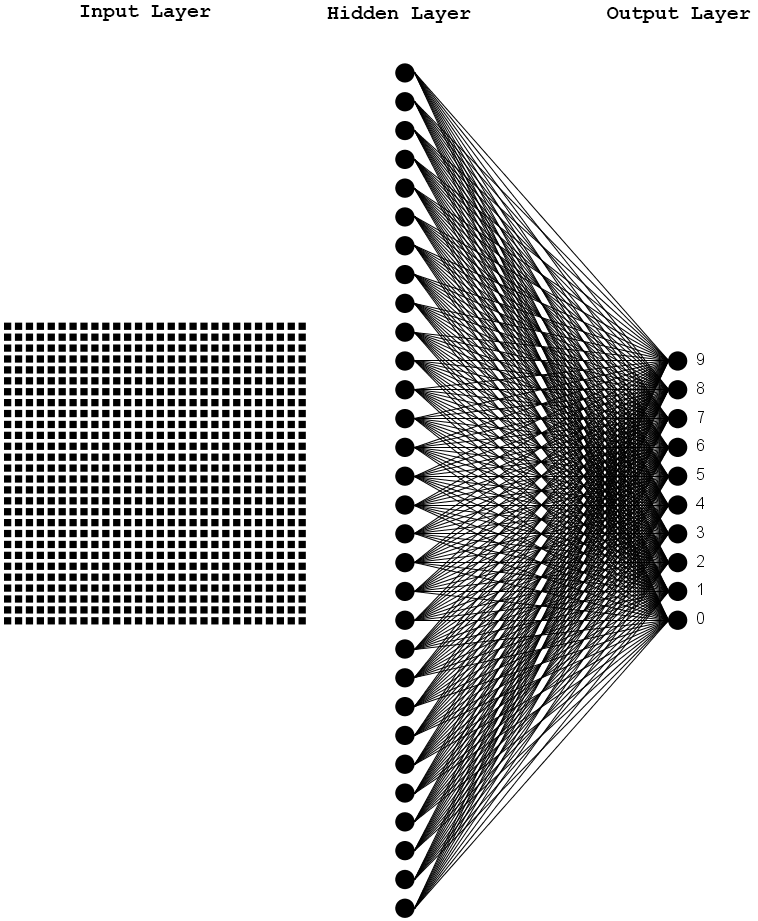
\includegraphics[scale=0.7]{Bilder/animation_network_default}
	\caption{Default Animation, welche über die Eingabe mit dem Wert $0$ aufgerufen wird.} 
	\label{fig:animation_network_default} 
\end{figure}

\noindent
Der Funktion $\mathtt{drawLayer()}$ werden die Parameter für die Größe des Radius $\mathtt{r}$ eines Neurons und des momentan ausgewählten Neurons $\mathtt{acitveNeuron}$ übergeben. Der Code für das Zeichnen der einzelnen Schichten ist dann gegeben durch:
\begin{Verbatim}[ frame         = lines, 
                  framesep      = 0.3cm, 
                  firstnumber   = 1,
                  labelposition = bottomline,
                  numbers       = left,
                  numbersep     = -0.2cm,
                  xleftmargin   = 0.8cm,
                  xrightmargin  = 0.8cm,
                ]
    drawLayer := procedure(r, activeNeuron) {
        gfx_setPenColor("BLACK");
        for(i in {1 .. #mNetwork}) {	
            for(j in {0 .. mNetwork[i]-1}) {
                if(activeNeuron == j && i ==1) {
                    gfx_setPenColorRGB( 1.0, 0.0, 0.0 );				
                    gfx_filledCircle((mSqrtAllPixel*12+300*i), ((mScreenSizeY-r*(3*mNetwork[i]-1))/2)+3*r*j, r);
                } else {
                    gfx_setPenColorRGB( 0.0, 0.0, 0.0 );
                    gfx_filledCircle((mSqrtAllPixel*12+300*i), ((mScreenSizeY-r*(3*mNetwork[i]-1))/2)+3*r*j, r);
				
                    if(i == #mNetwork) {			
                        gfx_textRight((mSqrtAllPixel*12+300*i)+30, ((mScreenSizeY-r*(3*mNetwork[i]-1))/2)+3*r*j, j);
                    }
                }
            }		
        }
    };
\end{Verbatim}
\begin{enumerate}
	\item Zeile 3-4: Für das Zeichnen der einzelnen Schichten werden die Schichten mit der korrespondierten Anzahl von Neuronen.
	\item Zeile 5-7: Das aktive Neuron auf dessen Betrachtung in der Animation fällt, wird durch die Farbe "rot" hervorgehoben.   
	\item Zeile 8-13: Alle nicht aktiven Neuronen werden schwarz abgebildet. Für die Ausgabeschicht wird zusätzlich der erwartete Ausgabewert abgebildet, wenn $\mathtt{i == \#mNetwork}$ (siehe Zeile 12-13).
\end{enumerate}
Die Berechnung der x-Koordinate für das abzubildende Neuron wird über \\[0.2cm]
\hspace*{1.3cm}
$
\begin{array}[t]{lclll}
	\mathtt{mSqrtAllPixel*12+300*i}
\end{array}
$ 
\\[0.2cm]
ermittelt. Dazu wird der der benötigte Bereich für die Eingabeschicht mittels $\mathtt{mSqrtAllPixel}*12$ berechnet, wobei für jede Iteration durch die Layer-Liste des Netzwerks 300px hinzukommen. Für die y-Koordinate ergibt sich die Formel \\[0.2cm]
\hspace*{1.3cm}
$
\begin{array}[t]{lclll}
	\mathtt{(mScreenSizeY-r*(3*mNetwork[i]-1))/2+3*r*j}.
\end{array}
$ 
\\[0.2cm]
Dabei wird der mittlere Abstand der grafischen Ausgabe einer Schicht zum Fensterrand in Abhängigkeit des Radius $r$ über $(\mathtt{mScreenSizeY}-r*(3*\mathtt{mNetwork[i]}-1))/2$ berechnet. Für jedes Neuron $j$ in der Schicht $i$ wird der Durchmesser $2*r$ des Neurons und der Abstand $r$ zum nächsten Neuron über $3*r*j$ addiert. \\

\noindent
Im nächsten Abschnitt wird die Implementierung der $\mathtt{drawConnection()}$-Funktion vorgestellt. Die Funktion verbindet jedes Neuron der Schicht $n$ mit jedem Neuron der Schicht $n+1$. Hierbei sind die Berechnung der Koordinaten $x_1$, $y_1$ sowie $x_2$, $y_2$ äquivalent zu den Berechnung der vorangegangenen $\mathtt{drawLayer()}$-Funktion.
\begin{Verbatim}[ frame         = lines, 
                  framesep      = 0.3cm, 
                  firstnumber   = 1,
                  labelposition = bottomline,
                  numbers       = left,
                  numbersep     = -0.2cm,
                  xleftmargin   = 0.8cm,
                  xrightmargin  = 0.8cm,
                ]
    drawConnection := procedure(r) {
        gfx_setPenColor("BLACK");
        for(i in {1 .. #mNetwork-1}) {	
            for(j in {0 .. mNetwork[i]-1}) {
                for(k in {0 .. mNetwork[i+1]-1}) {
                    if(i<#mNetwork) {
                        gfx_line((mSqrtAllPixel*12+300*i+r), ((mScreenSizeY-r*(3*mNetwork[i]-1))/2)+3*r*j, (mSqrtAllPixel*12+300*(i+1)-r), ((mScreenSizeY-r*(3*mNetwork[i+1]-1))/2)+3*r*k);
                    }	
                }
            }		
        }
    };
\end{Verbatim}
Als letztes wird die Funktion $drawNeuron$ diskutiert, welche ausgehend von den Gewichtungen und den Testdaten Bereiche mit höherer Relevanz farbliches hervorhebt. Die farbliche Unterteilung hat dabei die folgende Bedeutung.
\begin{center}
\begin{tabular}{lp{6cm}}
\textbf{Farbe}   & \textbf{Erklärung} \\
\hline \\
blau, grün & Bereich mit einer geringen Relevanz \\[0.2cm]
rot, gelb  & Bereich mit einer hohen Relevanz   \\
\end{tabular}
\end{center}
Für die unterschiedlichen Animationsmöglichkeiten muss an dieser Stelle unterschieden werden, ob die anzuzeigenden Daten nur die Gewichtungen, die Testdaten oder eine Kombination beider abbilden sollen. 